\chapter{Contributions}

\newcounter{treeline}

\newcommand{\treeroot}[1]{% Title
\node[above] at (0,0) {#1};%
\setcounter{treeline}{0}
}

\newcommand{\treeentry}[2]{% Title, Level
\draw[->] (#2-1,-\value{treeline}/2) -- (#2-1,-\value{treeline}/2-0.5) -- (#2+0.5,-\value{treeline}/2-0.5) node[right] {#1};
\stepcounter{treeline}
}

\newcommand{\altentry}[2]{% Title, Level
\draw[->] (#2-1,-\value{treeline}/2) -- (#2-1,-\value{treeline}/2-0.5) -- (#2+0.5,-\value{treeline}/2-0.5) node[right] {#1};
\foreach \x in {1,...,#2}
{   \draw (\x-1,-\value{treeline}/2) -- (\x-1,-\value{treeline}/2-0.5);
}
\stepcounter{treeline}
}

\textcolor{blue}{Andreas Bock}\\
\textcolor{green}{Johan Astborg}\\
\textcolor{red}{Both}\\

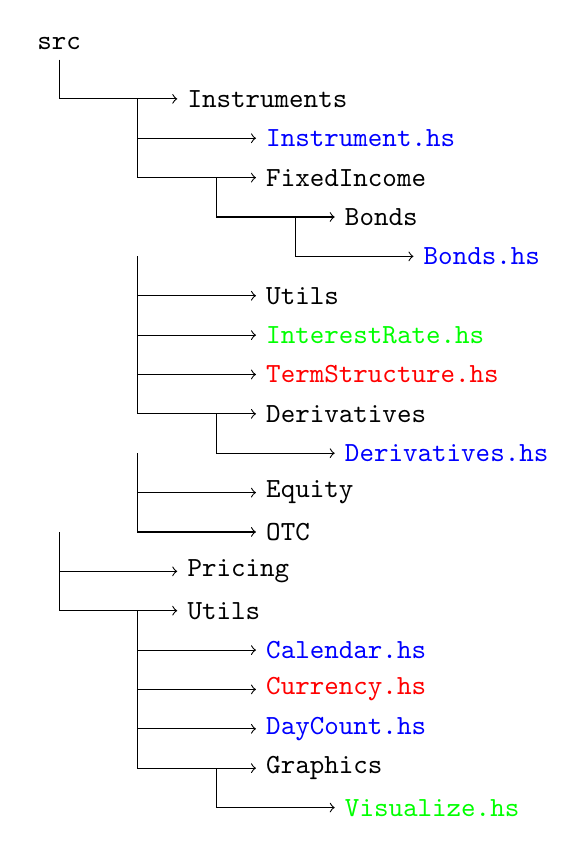
\begin{tikzpicture}
\tt
\treeroot{src}
\treeentry{Instruments}{1}
\treeentry{\color{blue} Instrument.hs}{2}
\treeentry{FixedIncome}{2}
\treeentry{Bonds}{3}
\treeentry{\color{blue} Bonds.hs}{4}
\treeentry{Utils}{2}
\treeentry{\color{green} InterestRate.hs}{2}
\treeentry{\color{red} TermStructure.hs}{2}
\treeentry{Derivatives}{2}
\treeentry{\color{blue} Derivatives.hs}{3}
\treeentry{Equity}{2}
\treeentry{OTC}{2}

\treeentry{Pricing}{1}
\treeentry{Utils}{1}
\treeentry{\color{blue} Calendar.hs}{2}
\treeentry{\color{red} Currency.hs}{2}
\treeentry{\color{blue} DayCount.hs}{2}
\treeentry{Graphics}{2}
\treeentry{\color{green} Visualize.hs}{3}
\end{tikzpicture}

\chapter{Source Code}

\input{src/HQL.hs}
\input{src/Utils/Calendar.hs}
\input{src/Utils/Currency.hs}
\input{src/Utils/DayCount.hs}
\input{src/Utils/Brownian.hs}
\input{src/Utils/Graphics/Visualize.hs}
\input{src/Instruments/Utils/InterestRate.hs}
\input{src/Instruments/Utils/TermStructure.hs}
\input{src/Instruments/FixedIncome/Bonds/Bonds.hs}
\input{src/Instruments/Derivatives/Derivatives.hs}

\chapter{\textsc{HQL} Documentation}

